\section{Test Case Generation using Deep Learning}

\subsection{CLgen}

Figure~\ref{fig:deeptune} shows the test case generation process.

\begin{itemize}
\item An initial seed corpus of OpenCL samples is mined from GitHub. An oracle compiler (LLVM 3.9) is used to reject samples were not well formed.
\item Corpus is preprocessed and encoded for training. A uniform code style is enforced for whitespace, braces, identifier names, etc.
\item LSTM networks model the vocabulary distribution over the encoded corpus.
\item The trained network is sampled to generate new programs.
\end{itemize}

\noindent In subsequent iterations, synthesized kernels may be used to augment the training corpus.

\begin{itemize}
\item Samples are synthesized by the network and pruned using the rejection filter.
\item The samples are mixed with kernels from the GitHub seed corpus.
\item These combined samples are labeled (synthetic or human), and used to train a classifier for human-or-robot.
\item The classifier is tested on unseen programs, and the accuracy is used as a fitness function for the model's parameters.
\item A GA mutates and evolves the best performing parameters.
\end{itemize}


\begin{figure}
  \centering
  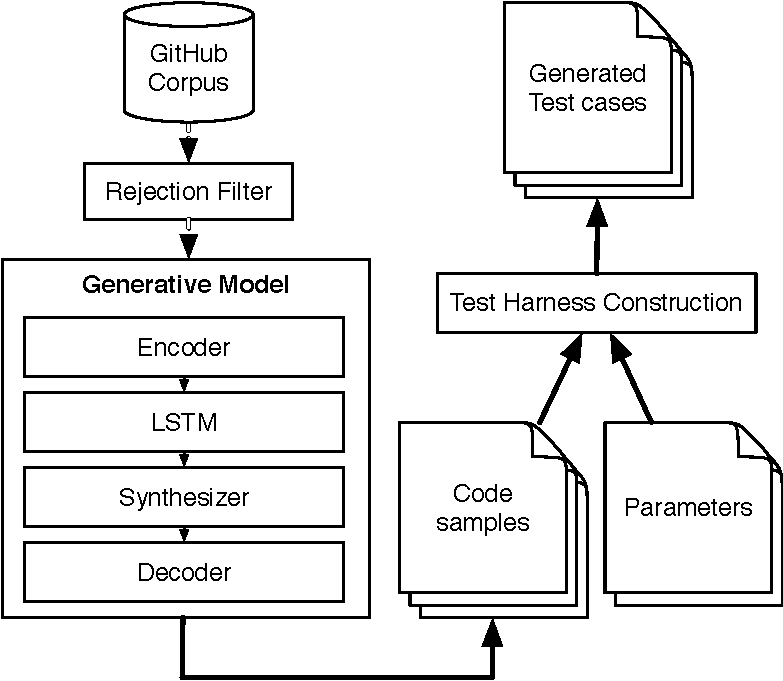
\includegraphics[width=.95\columnwidth]{img/clgen} %
  % \vspace{-2em}%
  \caption{%
    Test-case generation. A corpus of programs from GitHub is used to seed a generative model for program codes.%
  }%
  \label{fig:deeptune}
\end{figure}

\subsection{Test Case Execution}

At first, we used the test harness of CLSmith. However, this was too inflexible for our needs, requiring all kernels accept the same argument of a single \texttt{unsigned long} buffer. This prototype, in addition to being restricting, is not a common OpenCL use case (only XX\% of GitHub kernels have this prototype). Instead, we created cldrive, a tool to generate test harnesses for arbitrary OpenCL kernels.

Generate host code stub to compile kernel. If kernel compiles: parse AST, read function arguments, generate data inputs for arguments. Limited subset of data types supported: No structs, no irregular data types (this is just an implementation detail, and can be addressed with more dev time).
